
\section{Nvidia and GPGPU}

\subsection{Background}
GPUs with programmable shaders supporting floating point operations were the beginning of GPGPU.
It started by using graphics libraries to implement tensor operations.
One of the first implementations was a LU factorization in 2005 \cite{du2012cuda}.
Nvidia's CUDA platform was launched in 2008 to allow programming while ignoring the underlying graphical concepts.
Not alike alternatives --- such as OpenCL --- CUDA only works on Nvidia GPUs.
Its development has been tied to the development of the Tesla family of GPUs.
Just as GeForce is Nvidia's Desktop family, and Jetson their embedded family, Tesla is their HPC family.
Tesla was also the name of the microarchitecture in 2008, when they introduced CUDA.
Since then there has been a mostly continuous progress towards their latest microarchitecture, Pascal, presented in April 2016.
The biggest changes were introduced in the Fermi microarchitecture.

\subsection{Historical progress}
In 2010, Nvidia presented the Fermi microarchitecture, easing intensive use of GPUs in HPC.
Fermi introduced 40-bit memory addressing, and ISA support for up to 64-bit addressing \cite{nickolls2010gpu}.
It adopted the IEE 754-2008 floating point standard and enabled 64-bit floating point operations at only half of the throughput of FP32.
Fermi also introduced the current hierarchical cache with L1 cache connected to L2 cache and L2 to DRAM, with unified access to the three levels.
L2 and DRAM were enabled to access host CPU memory through PCIe.
The amount of L1 and L2 were configurable for the programmer, allowing a variable fixed fraction of shared memory.

The next generation, Kepler, was introduced in 2012 and introduced Dynamic Parallelism.
Dynamic Parallelism refers to enabling GPU threads to launch other threads (kernels launching kernels).
This provides the programming model with more flexibility.
This architecture is the one currently in use for GPGPU HPC tasks requiring 64-bit floating point precision.

The Maxwell microarchitecture, presented in 2014 introduced Unified Virtual Memory.
This was an important step in simplifying the programming model.
In this architecture, FP64 efficiency dropped by one order of magnitude.
Maxwell focused on graphics and per Watt performance.

The Pascal microarchitecture, presented in 2016, brings the features of the Kepler and Maxwell microarchitectures together.
It improves the Unified Virtual Memory model, thanks to page faulting and NVLink.
NVLink comes as an alternative to PCIe, but it does not replace it.
Pascal also brings back FP64 at high rates.
Memory bandwidth is improved thanks to the use of HBM2 memory.
FP16 operations are supported at double the rate of FP32 operations.
Pascal also introduces preemption at the instruction level.
All this comes with a reduction of the transistor size by using a 16nm FinFET technology.

The Volta microarchitecture was supposed to follow Maxwell.
However, lack of maturity of Hybrid Memory Cube versus High Bandwidth Memory, forced Nvidia to switch to the Pascal microarchitecture \cite{wccftech:volta}.
Volta systems will be installed in supercomputers in 2017, coming to the market in 2018.

\subsection{Recent evolution --- Pascal vs Kepler and Maxwell}

\begin{figure}[ht!]
    \centering
    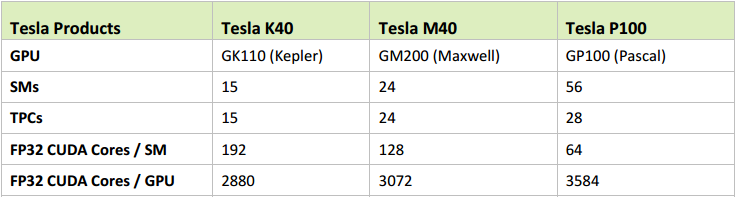
\includegraphics[width=\linewidth]{cuda_cores}
    \caption{Extract of table comparing Kepler, Maxwell and Pascal \cite{nvidia:pascalwhitepaper}}
    \label{fig:cuda_cores}
\end{figure}
The intent of this section is to try to make the recent architecture changes clear.
The relevant architectures for this comparison are Pascal, Maxwell and Kepler.
The chip representing Pascal is the GP100, installed in the Tesla P100.
Kepler has 2 representing chips, the GK110, part of the Tesla K40, and the GK210, part of the Tesla K80.
The K40 was announced in November 2013 and the K80 a year later, extending the life of Kepler.
This extended life was probably needed due to the lack of FP64 performance on the newer 2014 Maxwell architecture.
The top Maxwell chip GM200 was released in 2015 with the best performance if not considering FP64 performance.
Note that the letter preceding the chip model number, stands for the first letter of the architecture name.

In the more recent architectures a clearer hierarchical organization can be seen.
This is related to the GPGPU model presented in Section \ref{sec:gpgpu}.
GM200 and GP100 have both 6 Graphics Processing Clusters, formed by Texture Processing Clusters, formed by smaller Streaming Multiprocessors.
In contrast, the Kepler chips are structured as an array of 15 Streaming Multiprocessors with lots of processing cores each.
The number of CUDA Cores per Streaming Multiprocessor keeps decreasing.
The GK110, GM200, and GP100 have respectively 192, 128 and 64 FP32 CUDA Cores per Streaming Multiprocessor.
Kepler has a ratio of 1:3 FP64 to FP32 CUDA Cores, which was decreased to 1:32 in Maxwell.
Pascal has increased this ratio to 1:2 by having FP16 as part of the FP32 ALUs.
The number of Streaming Multiprocessors per GPU increases continuously, giving an increasing number of CUDA Cores per GPU.

The scheduler data path in Pascal is changed with respect to Kepler and Maxwell.
A big improvement in the scheduler in comparison to Maxwell is that each warp scheduler can dispatch two warp instructions per clock.
This allows for launching simultaneously two independent instructions (e.g. to ALU and Load/Store Unit).

Instruction-level preemption is a very relevant Pascal feature vs block-level preemption on the Maxwell and Kepler architectures.

Maxwell improved on the 64KB configurable shared memory/L1 cache of Kepler by increasing the available memory and creating separate spaces for shared memory and L1 cache.
The L2 cache in Pascal is not much larger with 4096KB, but the total L1 cache available per CUDA Core gets doubled.
The Register File Size per Streaming Multiprocessor has also been kept constant while decreasing the number of cores.
All this effectively increases the amount of fast cache and registers available per core, improving execution speed and concurrency.
GK210 already included double as much L1/shared memory per core vs GK110.

GK110 and GM200 had a 384-bit GDDR5 memory interface.
GP100 has a 4096-bit memory interface when using High Bandwidth Memory v2.
This makes GP100 have 3x the bandwidth of the Maxwell GM200 GPU even with HBM2 having a 3-4x slower clock.
Higher memory bandwidth improves work on larger data sets.

Kepler implemented atomic memory operations in software just like Fermi in a lock/update/unlock pattern.
Maxwell enabled native hardware support for atomic operations with 32-bit integers and 32-bit and 64-bit compare-and-swap operations.
Pascal allows atomics in Unified Memory, including 32 and 64-bit support for both integers and floats.

A constant in all this evolution is the TFLOPS/W improvement, effectively serving as a modification of Moore's law.
